\documentclass[10pt,a4paper]{article}
\usepackage{fontspec}
\usepackage{amsmath}
\usepackage{amsfonts}
\usepackage{amssymb}
\usepackage{graphicx}
\usepackage[left=1.00in, right=1.00in, top=1.00in, bottom=1.00in]{geometry}
\usepackage[colorlinks=true,
			linkcolor=blue]{hyperref}
\usepackage{cleveref}
\usepackage{minted}
\usepackage{lmodern}

\begin{document}
	\title{Assignment 3:\\Modified Sheath Conditions}
	\author{Daniel Celis Garza}
	\date{\today}
	\maketitle
	
	In order to model collisions within the sheath region we start from the equation for conservation of energy,
	\begin{align}
		\dfrac{1}{2} m_{i} v_{i}^{2} = \dfrac{1}{2} m_{i} v_{s}^{2} - e \phi(x)~.
	\end{align}
	Differentiating with respect to $x$, noting that $\dfrac{\mathrm{d} \phi}{\mathrm{d} x} = E$ and rearranging we obtain,
	\begin{align}
		m_{i} v_{i} \dfrac{\mathrm{d} v_{i}}{\mathrm{d} x} &= e E \nonumber\\
		\dfrac{\mathrm{d} v_{i}}{\mathrm{d} x} &= \dfrac{e}{m_{i} v_{i}} E.
	\end{align}
	In order to account for particle loss due to collisions we may add a term which subtracts from the velocity gradient. By dimensional analysis we know this term must be in $time^{-1}$, so we may assume it is directly proportional to the ion velocity $v_{i}$ and inversely proportional to a characteristic collision length, $L$. Thus making this new term have a value of $-\dfrac{v_{i}}{L}$, where we absorb any proportionality with $v_{i}$ into $L$. This adjustment also has the advantage of vanishing at large $L$, recuperating the case for no collisions. By defining $\hat{L} = \dfrac{L}{\lambda_{D}}$, using the same normalisations for all other quantities as described in assignment 1 and recalling the definition for $c_{s} = \sqrt{\dfrac{e T_{e}}{m_{i}}}$ we obtain the following normalised expression,
	\begin{align}
		\dfrac{c_{s}}{\lambda_{D}} \dfrac{\mathrm{d} \hat{v_{i}}}{\mathrm{d} \hat{x}} &= \dfrac{e T_{e}}{m_{i} c_{s} \lambda_{D} \hat{v_{i}}} \hat{E} - \dfrac{c_{s}}{\lambda_{D}} \dfrac{\hat{v_{i}}}{\hat{L}} \nonumber \\
		\dfrac{\mathrm{d} \hat{v_{i}}}{\mathrm{d} \hat{x}} &= \dfrac{e T_{e}}{m_{i} c_{s}^{2} \hat{v_{i}}} \hat{E} - \dfrac{\hat{v_{i}}}{\hat{L}} \nonumber \\
		\dfrac{\mathrm{d} \hat{v_{i}}}{\mathrm{d} \hat{x}} &= \dfrac{\hat{E}}{\hat{v_{i}}} - \dfrac{\hat{v_{i}}}{\hat{L}}~.
	\end{align}
	Which when solved replaces the static expression for $v_{i}$ of previous models.
	
	The ion velocity as a function of $x_{w}$ (adjusted $x$ found by finding where the current, $J = 0$ and subtracting that value from the $x$-array) is shown in \cref{fig:1}. Inset in \cref{fig:1} is the plot of the ion velocity at $x_{w} = 0$ as a function of $\log\left(\hat{L}\right)$.
	\begin{figure}
		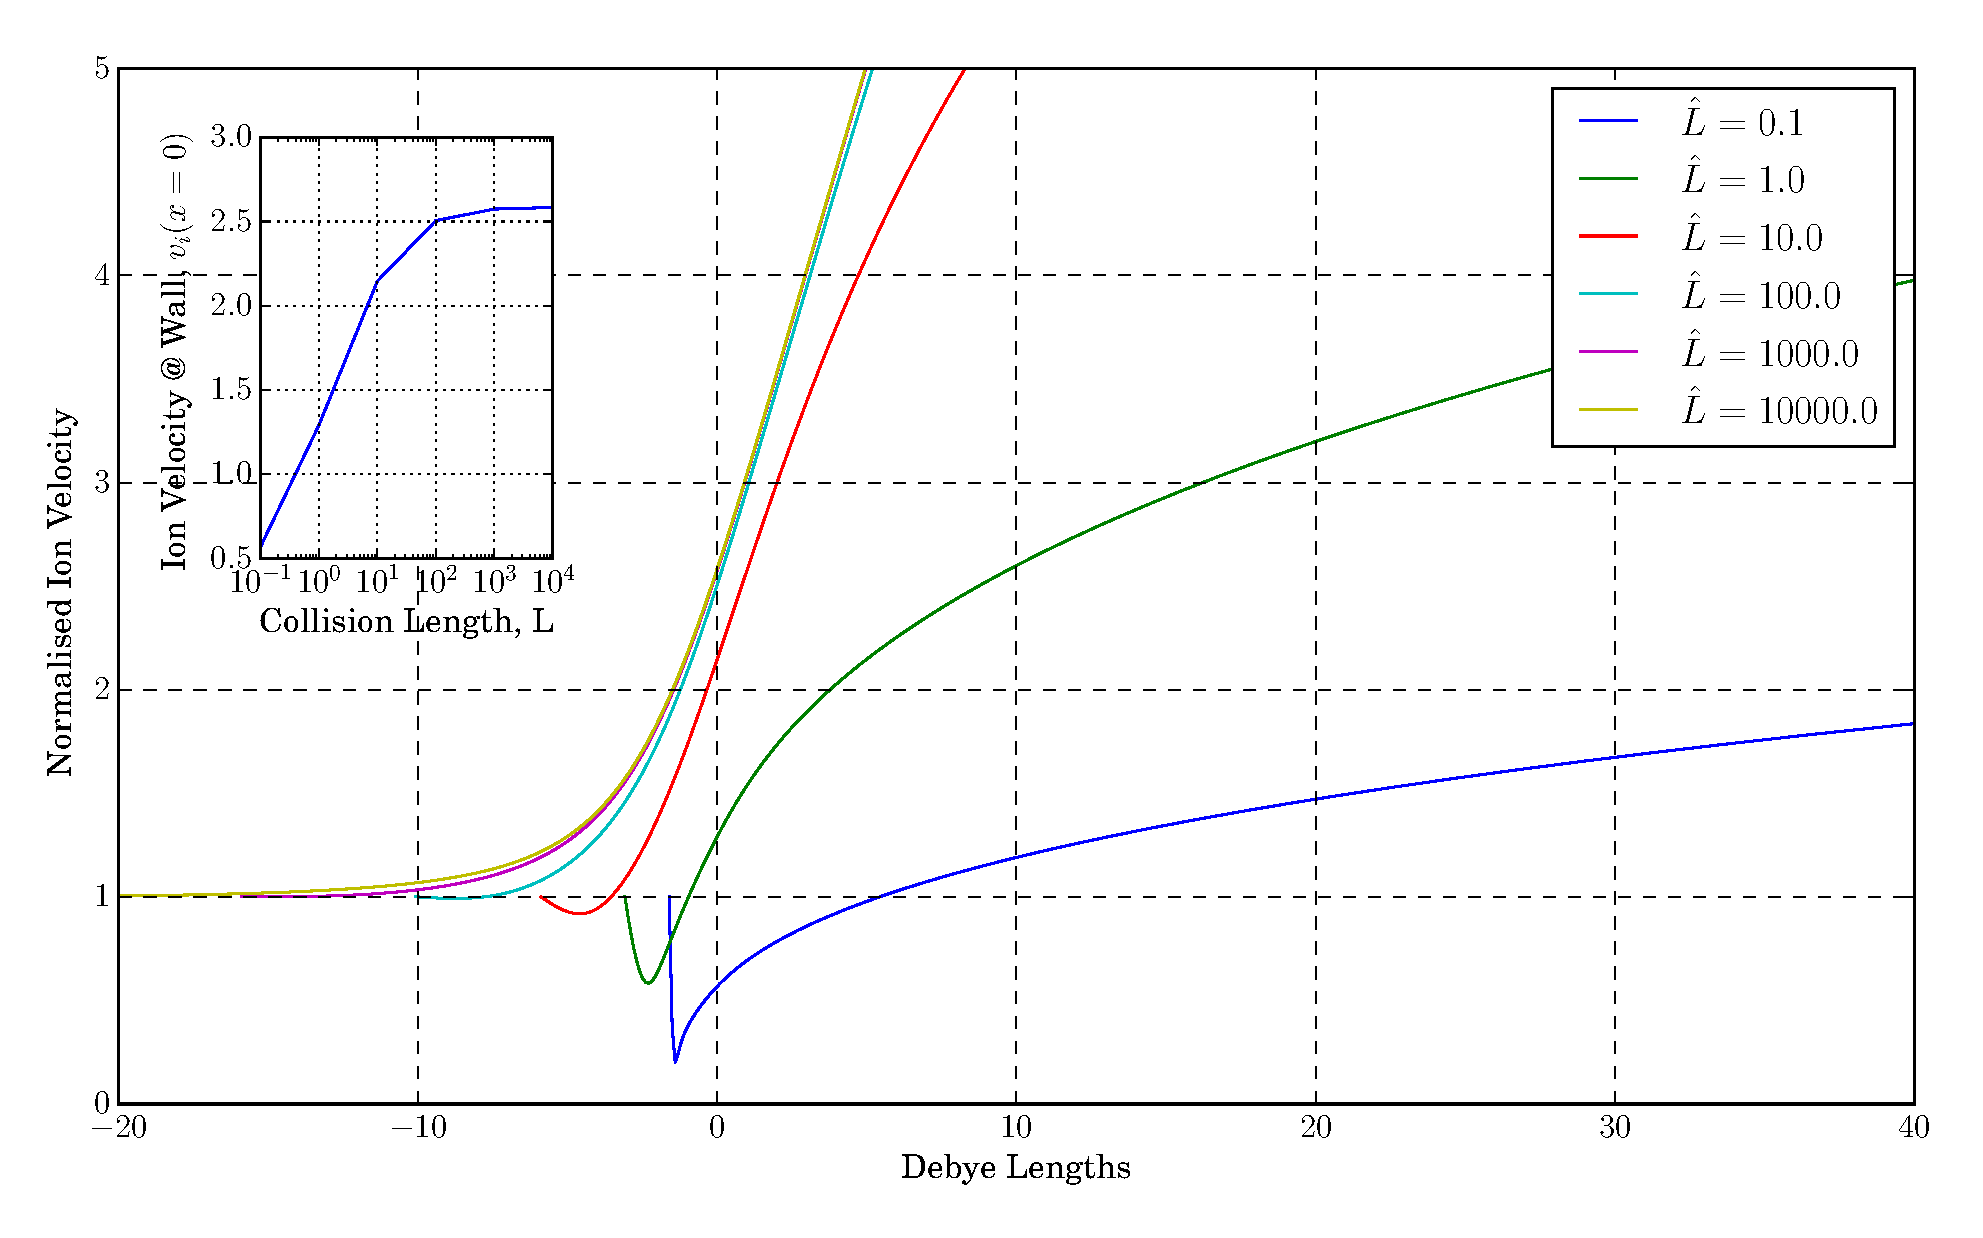
\includegraphics[width=\textwidth]{collisions.eps}
		\caption{Ion velocity as a function of $x_{w}$ for various values of $L$. Inset: Ion velocity at the wall as a function of $\log\left(\hat{L}\right)$.}
		\label{fig:1}
	\end{figure}
	It is interesting to note that 
	\begin{align}
		\lim\limits_{\hat{L} \rightarrow \infty} \left(\dfrac{\mathrm{d} \hat{v_{i}}}{\mathrm{d} \hat{x}} \right) = \dfrac{\hat{E}}{\hat{v_{i}}}~,
	\end{align}
	which after integration becomes,
	\begin{align}
		\left. \dfrac{1}{2} v_{i}^{2} \right|_{v_{i}}^{v_{s}} &= \int\hat{E}\mathrm{d}x \nonumber\\
		\dfrac{1}{2} \left(v_{s}^{2} - v_{i}^{2}\right) &= \hat{\phi}\\
		\hat{v_{i}} &= \sqrt{\hat{v_{s}^{2}} - 2 \hat{\phi}}~,
	\end{align}
	where $v_{s}$ is the ion velocity at the start of the sheath. This is the expression for the normalised ion velocity derived in assignment 1, and the explanation for the asymptotic behaviour observed in \cref{fig:1} as $\hat{L}$ increases.
	
	The source code is included.
	\inputminted[linenos = true,
	breaklines, 
	breakanywhere]{python}{dcg513_3.py}
\end{document}